\begin{document}
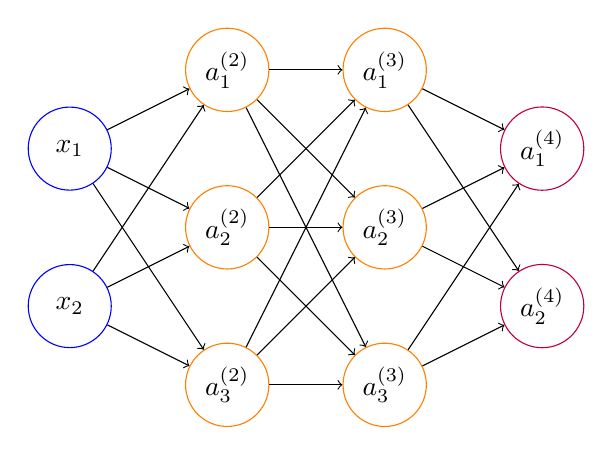
\begin{tikzpicture}
\node[circle,
minimum width =30pt ,
minimum height =30pt ,draw=blue] (1) at(0,2){$x_1$};
\node[circle,
minimum width =30pt ,
minimum height =30pt ,draw=blue] (2) at(0,0){$x_2$};
\node[circle,
minimum width =30pt ,
minimum height =30pt ,draw=orange] (3) at(2,-1){$a_3^{(2)}$};
\node[circle,
minimum width =30pt ,
minimum height =30pt ,draw=orange] (4) at(2,1){$a_2^{(2)}$};
\node[circle,
minimum width =30pt ,
minimum height =30pt ,draw=orange] (5) at(2,3){$a_1^{(2)}$};
\node[circle,
minimum width =30pt ,
minimum height =30pt ,draw=orange] (6) at(4,-1){$a_3^{(3)}$};
\node[circle,
minimum width =30pt ,
minimum height =30pt ,draw=orange] (7) at(4,1){$a_2^{(3)}$};
\node[circle,
minimum width =30pt ,
minimum height =30pt ,draw=orange] (8) at(4,3){$a_1^{(3)}$};
\node[circle,
minimum width =30pt ,
minimum height =30pt ,draw=purple] (9) at(6,2){$a_1^{(4)}$};
\node[circle,
minimum width =30pt ,
minimum height =30pt ,draw=purple] (10) at(6,0){$a_2^{(4)}$};
\draw[->] (1) --(3);
\draw[->] (1) --(4);
\draw[->] (1) --(5);
\draw[->] (2) --(3);
\draw[->] (2) --(4);
\draw[->] (2) --(5);
\draw[->] (3) --(6);
\draw[->] (3) --(7);
\draw[->] (3) --(8);
\draw[->] (4) --(6);
\draw[->] (4) --(7);
\draw[->] (4) --(8);
\draw[->] (5) --(6);
\draw[->] (5) --(7);
\draw[->] (5) --(8);
\draw[->] (6) --(9);
\draw[->] (6) --(10);
\draw[->] (7) --(9);
\draw[->] (7) --(10);
\draw[->] (8) --(9);
\draw[->] (8) --(10);
\end{tikzpicture}
\end{document}